\section{Auswertung}
\subsection{Bestimmung der RC-Konstanten durch die Entladungskurve}
In der Abbildung %\ref{fig:kurve}
ist die zur Ausmessung verwendete Entladungskurve des Kondensators zu sehen.
\begin{figure}[H]
  \centering
  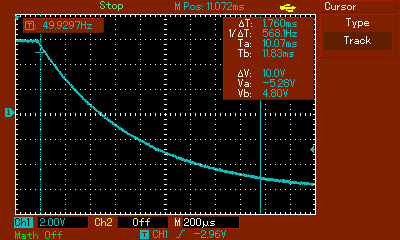
\includegraphics{kurve}
  \caption{Entladungskurve}
  \label{fig:kurve}
\end{figure}
In Tabelle \ref{tab:tabe1} sind die aus ihr gewonnenen Messwertpaare zusammen mit
dem Verhältniss $ \frac{U}{U_0} $ und dessen Logarithmus, welcher zur
Auswertung nötig ist, abzulesen.
\begin{table}[H]
  \centering
  \caption{Messwerte zur Bestimmung der RC-Konstanten}
  \label{tab:tabe1}
    \begin{tabular}{c c c c}
    \toprule
    $ t \: / \si{\milli\second} $ & $ U_C \: / \si {\volt} $ & $\frac{U_C}{U_0} $
    & $ \ln{\frac{U_C}{U_0}} $ \\
    \midrule
    0.000 & 12.00 & 1.000 & 0.000 \\
    0.080 & 10.88 & 0.907 & -0.098 \\
    0.160 & 9.84 & 0.820 & -0.198 \\
    0.240 & 8.96 & 0.747 & -0.292 \\
    0.320 & 8.16 & 0.680 & -0.386 \\
    0.400 & 7.44 & 0.620 & -0.478 \\
    0.480 & 6.80 & 0.567 & -0.568 \\
    0.560 & 6.16 & 0.513 & -0.667 \\
    0.640 & 5.68 & 0.473 & -0.748 \\
    0.720 & 5.20 & 0.433 & -0.836 \\
    0.800 & 4.72 & 0.393 & -0.933 \\
    0.880 & 4.32 & 0.360 & -1.022 \\
    0.960 & 4.00 & 0.333 & -1.099 \\
    1.040 & 3.68 & 0.307 & -1.182 \\
    1.120 & 3.36 & 0.280 & -1.273 \\
    1.200 & 3.12 & 0.260 & -1.347 \\
    1.280 & 2.88 & 0.240 & -1.427 \\
    1.360 & 2.64 & 0.220 & -1.514 \\
    1.440 & 2.48 & 0.207 & -1.577 \\
    1.520 & 2.32 & 0.193 & -1.643 \\
    1.600 & 2.16 & 0.180 & -1.715 \\
    1.680 & 2.00 & 0.167 & -1.792 \\
    1.760 & 2.00 & 0.167 & -1.792 \\

      \bottomrule
    \end{tabular}
\end{table}

